\documentclass[bachelor, och, referat, times]{SCWorks}

% параметр - тип обучения - одно из значений:
%    spec     - специальность
%    bachelor - бакалавриат (по умолчанию)
%    master   - магистратура
% параметр - форма обучения - одно из значений:
%    och   - очное (по умолчанию)
%    zaoch - заочное
% параметр - тип работы - одно из значений:
%    referat    - реферат
%    coursework - курсовая работа (по умолчанию)
%    diploma    - дипломная работа
%    pract      - отчет по практике
%    pract      - отчет о научно-исследовательской работе
%    autoref    - автореферат выпускной работы
%    assignment - задание на выпускную квалификационную работу
%    review     - отзыв руководителя
%    critique   - рецензия на выпускную работу
% параметр - включение шрифта
%    times    - включение шрифта Times New Roman (если установлен)
%               по умолчанию выключен 



\usepackage[colorlinks=false, pdfborder={0 0 0}]{hyperref}  % убирает и цвет, и рамки
\usepackage[T2A]{fontenc}
\usepackage[utf8]{inputenc}
\usepackage[english,russian]{babel}
\usepackage{graphicx}
\usepackage[sort,compress]{cite}
\usepackage{amsmath}
\usepackage{amssymb}
\usepackage{amsthm}
\usepackage{fancyvrb}
\usepackage{longtable}
\usepackage{array}
\usepackage{minted}
\usepackage{tempora}
\usepackage{listings}
\usepackage{verbatim}



\newcommand{\eqdef}{\stackrel {\rm def}{=}}
\newcommand{\No}{\textnumero}
\newtheorem{lem}{Лемма}
\setminted{style=bw,
	linenos=true,
	breaklines=true,
	numbersep=5pt,
	tabsize=2,
	fontsize=\small,
	bgcolor=white}
\setmintedinline{style=bw,
	bgcolor=white,
	fontsize=\normalsize
	}


%убирание преносов слов
\tolerance = 1
\emergencystretch = \maxdimen
\hbadness = 10000

\newcommand{\eqdef}{\stackrel {\rm def}{=}}

\newtheorem{lem}{Лемма}

\begin{document}
    
   % Кафедра (в родительном падеже)
    %\chair{математической кибернетики и компьютерных наук}
    \chair{информатики и программирования}
    % Тема работы
    \title{Анализ сложности быстрой и пирамидальной сортировок}
    
    % Курс
    \course{2}
    
    % Группа
    \group{211}
    
    % Факультет (в родительном падеже) (по умолчанию "факультета КНиИТ")
    \department{факультета компьютерных наук и информационных технологий}
    
    % Специальность/направление код - наименование
    
    \napravlenie{02.03.02 "--- Фундаментальная информатика и информационные технологии}
    
    % Для студентки. Для работы студента следующая команда не нужна.
    \studenttitle{студентки}
    
    % Фамилия, имя, отчество в родительном падеже
    \author{Никитенко Яны Валерьевны}
    
    % Заведующий кафедрой 
    %\chtitle{доцент, к.\,ф.-м.\,н.}
    %\chname{С.\,В.\,Миронов}
    % Научный руководитель (для реферата преподаватель проверяющий работу)
    %\satitle{доцент, к.\,ф.-м.\,н.} %должность, степень, звание
    %\saname{А.\,П.\,Грецова}
    % Руководитель ДПП ПП для цифровой кафедры (перекрывает заведующего кафедры)
    % \chpretitle{
    %     заведующий кафедрой математических основ информатики и олимпиадного\\
    %     программирования на базе МАОУ <<Ф"=Т лицей №1>>
    % }
    % \chtitle{г. Саратов, к.\,ф.-м.\,н., доцент}
    % \chname{Кондратова\, Ю.\,Н.}
    \date{2025}
    
    
    % Руководитель практики от организации (руководитель для цифровой кафедры)
    %\patitle{доцент, к.\,ф.-м.\,н.}
    %\paname{С.\,В.\,Миронов}
    
    % Руководитель НИР
    %\nirtitle{доцент, к.\,п.\,н.} % степень, звание
    %\nirname{В.\,А.\,Векслер}
    
    % Семестр (только для практики, для остальных типов работ не используется)
    %\term{2}
    
    % Наименование практики (только для практики, для остальных типов работ не
    % используется)
    %\practtype{учебная}
    
    % Продолжительность практики (количество недель) (только для практики, для
    % остальных типов работ не используется)
    %\duration{2}
    
    % Даты начала и окончания практики (только для практики, для остальных типов
    % работ не используется)
    %\practStart{01.07.2022}
    %\practFinish{13.01.2023}
    
    % Год выполнения отчета
   
    
    \maketitle

    
    
    % Включение нумерации рисунков, формул и таблиц по разделам
    % (по умолчанию - нумерация сквозная)
    % (допускается оба вида нумерации)
    %\secNumbering

    
    
   \tableofcontents
    
    % Раздел "Обозначения и сокращения". Может отсутствовать в работе
    %\abbreviations
    %\begin{description}
    %    \item $|A|$  "--- количество элементов в конечном множестве $A$;
    %    \item $\det B$  "--- определитель матрицы $B$;
    %    \item ИНС "--- Искусственная нейронная сеть;
    %    \item FANN "--- Feedforward Artifitial Neural Network
    %\end{description}
    
    % Раздел "Определения". Может отсутствовать в работе
    %\definitions
    
    % Раздел "Определения, обозначения и сокращения". Может отсутствовать в работе.
    % Если присутствует, то заменяет собой разделы "Обозначения и сокращения" и "Определения"
    %\defabbr
    

    \section{Быстрая сортировка}
    \subsection{Текст программы}


    \begin{verbatim}
   //  Для опорного элемента и разделеения массива элемента
int partition(vector<int>& arr, int low, int high) {

    
    int pivot = arr[high]; // Выбор опорной точки

   
    int i = low - 1; // Индекс наименшьего элемента распологается 
    справа от опорного элемнта

        // Прохождение arr[low..high] и перемещещние все меньших
       // элементы слева. Элементы от low до  high
       // i уменьшается после каждой итерации
    for (int j = low; j <= high - 1; j++) {
        if (arr[j] < pivot) {
            i++;
            swap(arr[i], arr[j]);
        }
    }

    swap(arr[i + 1], arr[high]); // Передвижение опорного элемента 
    после меньших элементов
    return i + 1;   // Возвращение позиций 
}
//

// Функция быстрой сортировки
void quickSort(vector<int>& arr, int low, int high) {
    while (low < high) {
        int pi = partition(arr, low, high); // Возвращает индекс опорного элемента

        // Рекурсивные вызовы для меньших и больших элементов
        if (pi - low < high - pi) {
            quickSort(arr, low, pi - 1);
            low = pi + 1; // Избегаем переполнения стека
        }
        else {
            quickSort(arr, pi + 1, high);
            high = pi - 1; // Избегаем переполнения стека
        }
    }
}
//
 \end{verbatim}


 \subsection{Анализ сложности}
 Общая сложность:
Для 2-х вложенных циклов общая сложность равна: (t + m) = O(n), 
Для внешнего while сложность: O(kn), где n – общее кол-во элементов, k – кол-во повторений внешнего цикла.
Тогда общая сложность по правилу суммы: O(max(kn,1,1)) = O(kn).
Если массив отсортирован, то в лучшем случае мы просто пройдёмся по его n элементам. Сложность равна O(nlogn), так как мы делим каждый раз при рекурсивном вызове массив пополам, и всего таких случаев log2 n.
Согласно первой теореме:
\begin{figure} [H]
        \centering
    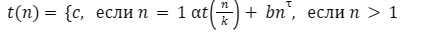
\includegraphics[width=0.50\linewidth]{Снимок экрана 2025-08-10 214444.png}
    \label{fig:first}
    \end{figure}

    построим реккурентное соотношение:


    \begin{figure} [H]
        \centering
    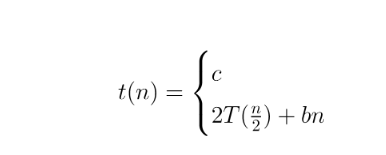
\includegraphics[width=0.50\linewidth]{Снимок экрана 2025-08-10 214221.png}
    \label{fig:first}
    \end{figure}

    Где a = 2 – кол-во подзадачи, порождаемых рекурсивной веткой, 
    n/k – размер подзадач, k = 2 – постоянная величина.

    Трудоемкость рекурсивного перехода имеет порядок $O(n), \tau  = 1.$
Значит по следствию теоремы для лучшего случая $ t(n) = O(n^\tau log_kn) = O(nlogn).$


В худшем случае опорный элемент каждый раз оказывается 
самым большим или самым маленьким элементом, 
что приводит к неравномерному разделению массива. 

Каждый раз опорный элемент оказывается таким, 
что один из подмассивов пуст, а другой содержит все элементы, кроме опорного. 
Если массив изначально отсортирован (или отсортирован в обратном порядке), 
каждый раз после разделения один из подмассивов 
будет содержать n - 1 элементов. 

Таким образом, количество уровней рекурсии будет n. 
На каждом уровне рекурсии мы выполняем O( n ) операций по разделению массива 
и сравнению элементов. В сумме на всех уровнях это дает O($n_2$).

Для худшего случая получим t(n) = O($n_2$).

Быстрая сортировка эффективна, 
когда по обеим сторонам от опорного элемента лежит равное количество элементов.



\section{Пирамидальная сортировка}
\subsection{Текст программы}

\begin{verbatim}
// Для создания кучи поддерева с корнем в узле i, который
// индекс в arr[]. n — размер кучи
void heapify(int arr[], int n, int i) {
    int largest = i; // Инициализируем наибольший элемент как корень
    int l = 2 * i + 1; // левый = 2*i + 1
    int r = 2 * i + 2; // правый = 2*i + 2

    // Если левый дочерний элемент больше корня
    if (l < n && arr[l] > arr[largest])
        largest = l;
    //

    // Если правый дочерний элемент больше, 
    чем наибольший элемент на данный момент
    if (r < n && arr[r] > arr[largest])
        largest = r;
    //

    // Если наибольший элемент не корень
    if (largest != i) {
        swap(arr[i], arr[largest]); // Перестановка
        heapify(arr, n, largest); // Рекурсивная группировка 
        соответствующего поддерево
    }
    //
}
//

// Основная функция сортировки кучи
void heapSort(int arr[], int n) {
    // Построение кучи (перегруппировка массива)
    for (int i = n / 2 - 1; i >= 0; i--)
        heapify(arr, n, i);

    // Извлечение элементов из кучи
    for (int i = n - 1; i >= 0; i--) {
        swap(arr[0], arr[i]); // Перемещение текущего элемента

        // Вызов на усеньшенной куче
        heapify(arr, i, 0);
    }
}
//


 \end{verbatim}

 \subsection{Анализ сложности}

 Сортировка основана на построении кучи. Свойства кучи:
Узел всегда больше своих потомков;
На последнем уровне элементы располагаются слева направо, пока онине закончатся.

Т.к. куча – это бинарное дерево, то его высота не больше, чем $log_2 N$, 
а значит временная сложность функции построения кучи равна O(logN).

В самом цикле сортировки мы проходимся по N элементов, 
значит общая сложность алгоритма O(N logN).
Эффективность алгоритма уменьшается, 
если все большие значения находятся в одной части пирамиды.



    \appendix
     
\end{document}